% paper/main.tex — master LaTeX document for the Level 1.5 InEKF paper.
%
% Build:
%   cd paper && pdflatex main && bibtex main && pdflatex main && pdflatex main
%
% Template notes:
%   Currently uses a generic article class. To switch to a venue-specific
%   template (NeurIPS 2026, ICLR 2026, ICML 2026), replace the preamble
%   below with the venue's style file and adjust \title/\author accordingly.

\documentclass[11pt]{article}

\usepackage[a4paper,margin=1in]{geometry}
\usepackage{amsmath,amssymb,amsthm}
\usepackage{graphicx}
\usepackage{booktabs}
\usepackage{hyperref}
\usepackage{xcolor}
% \usepackage{algorithm}      % uncomment when a pseudocode algorithm is added
% \usepackage{algpseudocode}  % needs texlive-science package
\usepackage{microtype}
\usepackage{natbib}

\hypersetup{
  colorlinks=true,
  linkcolor=blue!60!black,
  citecolor=blue!60!black,
  urlcolor=blue!60!black,
}

% Figure placement directory
\graphicspath{{../paper_figures/}}

\title{
  Parallel Invariant EKF on SO(2): \\
  Heteroscedastic Kalman Correction for MapFormer's Cognitive Maps
}

\author{
  Prash Rangarajan \\
  Paul G.\ Allen School of Computer Science \& Engineering \\
  University of Washington \\
  \texttt{prashr@cs.washington.edu}
}

\date{\today}

\begin{document}

\maketitle

\begin{abstract}
  MapFormer~\citep{rambaud2025mapformer} solves the clean aliased-observation
cognitive-map task nearly to ceiling (0.99+ next-token accuracy) by replacing
RoPE's fixed positional rotations with input-dependent rotations in
$\mathrm{SO}(2)$. The paper's reported task is therefore not where additional
mechanism is needed. This work asks instead: what happens when we push
MapFormer into regimes the paper did not test --- action noise, true
(non-aliased) landmarks, out-of-distribution sequence lengths, and calibrated
uncertainty --- and can classical Lie-group filtering help?
\par
We contribute a family of parallel Invariant Extended Kalman Filter
extensions to the MapFormer-WM backbone, implementable using either FFT
convolution (constant gain) or scalar Hillis-Steele associative scan
(time-varying gain), both matching MapFormer's $\mathcal{O}(\log T)$ scan
depth. Our main variant --- \textbf{Level 1.5 InEKF} --- uses a constant
learnable prior covariance $\Pi$ and a per-token measurement noise $R_t$
output by a small MLP, yielding a heteroscedastic Kalman gain
$K_t = \Pi / (\Pi + R_t)$ computable in a single affine scan.
\par
On the paper's clean aliased task, Level 1.5 matches MapFormer-WM within
noise and closes the NLL gap (reflecting calibrated confidence at landmark
tokens). The architectural wins appear outside the paper's tested regime:
under 10\% action noise at $4\times$ training length, Level 1.5 beats
MapFormer-WM by \textbf{+11\,pp} with half the NLL; with 200 true landmarks,
Level 1.5 beats MapFormer-WM by \textbf{+11\,pp} at $T{=}512$ OOD with roughly
half the NLL. We additionally confirm a negative result from the MapFormer
paper's Appendix A.5 at our scale: generic diagonal-$A$ Mamba-style selective
SSMs fail the cognitive-map task (accuracy $\approx 0.57$ across configs).
Honest hippocampal correspondence analysis partially falsifies biological
predictions: MapFormer does not produce hexagonal grid cells (architecturally
forced), and the learned $R_t$ does not follow the predicted Bayesian
informativeness ordering. All methods preserve MapFormer's parallel
path-integration scan.

\end{abstract}

\section{Introduction}
\label{sec:intro}

MapFormer~\citep{rambaud2025mapformer} is the current state-of-the-art
Transformer architecture for learning cognitive maps of structured
environments. By replacing RoPE's~\citep{su2021roformer} fixed positional
rotations with \emph{input-dependent} rotations driven by the action stream,
MapFormer performs path integration in the Lie algebra of $\mathrm{SO}(n)$ via
cumulative sum, preserving Transformers' $\mathcal{O}(\log T)$ parallelism
while recovering TEM-style~\citep{whittington2022tem-t} structural
disentanglement. On the authors' aliased-observation next-token prediction
benchmark, MapFormer-EM reaches 0.999 in-distribution accuracy and
MapFormer-WM reaches 0.955; neither leaves meaningful headroom on that
specific task.

\paragraph{The authors' task is therefore solved.} A paper that claimed ``we
improve on MapFormer's own task by an additional fraction of a percentage
point'' would be uninteresting, and we do not make that claim. Instead, this
paper takes MapFormer's benchmark as a confirmed starting point and asks
whether the surrounding architectural neighbourhood holds larger,
currently-unrealised wins:

\begin{enumerate}
  \item \textbf{Action noise}, which the paper does not study. Real
  navigation is noisy; if the path-integration estimate drifts, what does the
  architecture do?
  \item \textbf{True (non-aliased) landmarks}, also not studied in the paper.
  The paper's observation vocabulary maps 16 symbols randomly to 4096 grid
  cells, so every observation is ambiguous by construction. Environments
  with a small fraction of uniquely-identifying landmarks should let the
  model snap back to a precise position estimate --- but only if it has a
  mechanism for doing so.
  \item \textbf{Out-of-distribution sequence length}, tested only to $T{=}512$
  in the paper. Classical Kalman filtering has provable bounded-error
  guarantees under observability; do MapFormer-family architectures with
  explicit state correction inherit these guarantees empirically?
  \item \textbf{Calibration}, not measured in the paper. Point accuracy can
  saturate without the model knowing \emph{when} to be confident. A model
  that outputs per-token uncertainty should be able to sharpen its
  distribution at informative tokens and broaden it elsewhere.
\end{enumerate}

\paragraph{Our contribution} is a family of parallel Invariant Extended
Kalman Filter (InEKF, after \citealp{barrau2017inekf}) extensions to
MapFormer that add explicit state-correction machinery without sacrificing
$\mathcal{O}(\log T)$ scan depth. We build on MapFormer-WM (the weaker of the
paper's two variants) because its single-branch input-dependent rotation
admits a clean coupling between the filter's corrected state $\hat\theta$ and
the attention stream; a port to MapFormer-EM is mechanically straightforward
but not explored here. We report multi-seed MapFormer-EM numbers as an
upper-bound reference throughout.

\paragraph{Four findings.}

\begin{enumerate}
  \item \textbf{A fully-parallel InEKF on $\mathrm{SO}(2)$ is practical.} The
  closed-form scalar DARE yields a steady-state gain implementable as an
  FFT-based convolution (Level 1); adding a per-token learned measurement
  noise $R_t$ yields time-varying gain implementable as a scalar
  Hillis-Steele affine scan (Level 1.5); a full heteroscedastic prior
  $\Pi_t$ requires a M\"obius-matrix scan (Level 2). All three match the
  parallelism profile of Mamba-family selective SSMs~\citep{gu2024mamba}.
  \item \textbf{Simpler filters win.} Level 2 is strictly more expressive
  than Level 1.5 yet performs measurably worse in our experiments. We
  diagnose this as optimisation difficulty from the M\"obius scan, since
  replacing it with a learnable scalar while retaining the heteroscedastic
  gain (Level 1.5) recovers all the benefits at a fraction of the compute.
  \item \textbf{On the paper's clean task, Level 1.5 essentially matches
  MapFormer-WM.} Accuracy 1.000 vs 0.990 at $T{=}128$, 0.995 vs 0.921 at
  $T{=}512$ ($4\times$ OOD), with NLL 0.000 vs 0.031 --- the NLL gap reflects
  calibrated confidence at landmark tokens rather than a raw accuracy gap.
  \item \textbf{In the paper's untested regimes, Level 1.5 opens measurable
  gaps.} Under 10\% action noise at $T{=}512$ (4$\times$ OOD), Level 1.5
  beats MapFormer-WM by +11\,pp (0.851 vs 0.739). With 200 true landmarks
  added to the grid at $T{=}512$ OOD, Level 1.5 again beats MapFormer-WM by
  +11\,pp (0.821 vs 0.715). Both differences hold across three training
  seeds and are accompanied by roughly $2\times$ lower NLL, matching the
  classical filtering story: bounded error under observability, sharper
  posteriors at informative tokens.
\end{enumerate}

\paragraph{What this work is not.} We are not introducing a new benchmark;
we are not scaling to large models; and we are not claiming to have beaten
a state-of-the-art that was at 0.99+ before we started. We are demonstrating
that a classical robotics tool (the Invariant EKF), parallelised to match
MapFormer's depth profile, extends MapFormer's reach into regimes the paper
acknowledged it did not test.

\section{Related Work}
\label{sec:related}

\paragraph{Cognitive maps in neural models.} The Tolman-Eichenbaum Machine
(TEM)~\citep{whittington2020tem} introduced transformer-adjacent models of
the hippocampal formation that factorize ``structure'' (position) from
``content'' (sensory observations). Its transformer variant,
TEM-T~\citep{whittington2022tem-t}, reformulated this as a transformer with
action-dependent position updates. MapFormer~\citep{rambaud2025mapformer}
is the most recent development in this line, replacing TEM-T's sequential
rotation updates with a parallel cumulative-sum Lie-algebra path integration.

\paragraph{Transformer position encodings.} RoPE~\citep{su2021roformer}
rotates queries/keys by angles that are a fixed function of token index;
CoPE~\citep{golovneva2024cope} gates rotations by content to compress
relative distance; TAPE~\citep{zhu2025tape} updates positional embeddings
after attention. None of these adapt rotations to an external action
signal. MapFormer's core contribution is precisely this adaptation. Per
the MapFormer paper's own Table 2, all three fail the 2D-navigation task
at a single layer (RoPE 0.16, TAPE 0.32, CoPE 0.74 IID) while
MapFormer-WM saturates at $\approx 1.00$.

\paragraph{Cognitive-map filtering frameworks.} The Clone-Structured
Cognitive Graph (CSCG;~\citealp{george2021cscg}) uses discrete latent
states --- ``clones'' --- to disambiguate aliased observations,
representing the Bayesian posterior over position as a categorical
distribution. This is a forward-model strategy: given a position, predict
the expected observation distribution. Classical navigation filters
(EKF, UKF, Invariant EKF) use inverse models: given an observation,
infer the implied position. Our analysis frames these as complementary
inductive biases for the correction mechanism; our main Level~1.5
variant is inverse-model-based, while our Predictive-Coding variant is
forward-model-based.

\paragraph{Invariant filtering on Lie groups.}
\citet{barrau2017inekf} introduced the Invariant Extended Kalman Filter,
showing that on matrix Lie groups with group-affine dynamics the error
admits autonomous (state-independent) dynamics, enabling bounded-error
guarantees under observability. \citet{markovic2017wrapping} showed that
on $\mathrm{SO}(2)$ the wrapped-innovation EKF is mathematically
equivalent to the full Lie-Group EKF, which we exploit for correctness
at minimal implementation cost.

\paragraph{Parallel Bayesian filtering.}
\citet{sarkka2021parallel} introduced parallelizable Bayesian filters
via associative scan, enabling $\mathcal{O}(\log T)$ depth for
linear-Gaussian state-space models. Subsequent work extended this to
nonlinear iterated filters. Mamba~\citep{gu2024mamba} brought such scans
to deep learning as a replacement for attention; our Level~2 design uses
the same associative-scan primitive on M\"obius $2\times 2$ matrices,
and Level~1.5 uses a simpler scalar-affine variant.

\paragraph{Predictive coding.} Rao \& Ballard (1999) formalized the
``prediction error as signal'' view: top-down predictions compared
against bottom-up signals give error signals that drive state updates.
Friston's Free-Energy Principle generalizes this. We implement a
predictive-coding variant of MapFormer that uses an MLP forward model
from $(\cos\theta, \sin\theta)$ to expected observation embedding, with
prediction error driving an additive state correction. We find it
complementary to InEKF's inverse-model approach --- stronger at aliased
aggregation, weaker at sharp landmark measurement.

\paragraph{State-space language models and the Mamba-Kalman connection.}
Selective SSMs \citep{gu2024mamba} use associative scans for
parallel-friendly recurrence. \citet{wang2025mamba-kalman} prove an
isomorphism: Mamba's selective SSM is equivalent to a time-varying
linear Kalman filter under an appropriate parameterization. Our Level~1.5
is a specialisation of this: a 1-D Mamba block with three additional
constraints --- (i) Kalman-ratio gain parameterization
$K_t = \Pi/(\Pi + R_t)$, (ii) Lie-group-correct wrapping of innovations,
(iii) decoupled path-integration + correction scans. We demonstrate
empirically that this specialisation is \emph{discoverable} from
gradient descent while generic selective SSMs are not, in the
cognitive-map regime.

\paragraph{Heteroscedastic Kalman filtering.} Learning per-observation
measurement noise is a well-studied idea in classical filtering (the
``innovation covariance estimation'' literature of the 1970s--80s) and
in modern learned-filter work such as KalmanNet (Revach et al., 2022).
Our Level~1.5 differs from these by coupling heteroscedastic $R_t$ with
fixed covariance $\Pi$, implemented via a single scalar associative
scan. This makes it architecturally lighter than KalmanNet while
retaining the key per-token gain adaptation.

\section{Methods}
\label{sec:methods}

\subsection{Notation and Setup}

We work on the 2D torus GridWorld from~\citet{rambaud2025mapformer}. An
environment of size $N \times N$ (typically $N{=}64$) assigns to each cell
an observation type from $K + 1$ symbols: $K$ regular types plus a blank
token $B$. A fraction $p_\mathrm{empty}$ of cells are blank. Optionally,
$L$ additional cells carry unique single-use landmark tokens (disjoint
from the $K$ regular types).

The agent emits an interleaved trajectory
\begin{equation}
  s = (a_1, o_1, a_2, o_2, \ldots, a_T, o_T)
\end{equation}
with actions $a_t \in \{\uparrow,\downarrow,\leftarrow,\rightarrow\}$
sampled over directed walks ($k$ steps per chosen direction,
$k \in \{1,\ldots,10\}$) and observations $o_t$ determined by the
obs-map at the agent's current cell after applying $a_t$. We train on
$\sim$1M sequences ($T{=}128$ steps, batch size 128, AdamW
$\mathrm{lr}{=}3\!\times\!10^{-4}$, weight decay 0.05, linear LR decay).

\paragraph{Task.} Self-supervised next-token prediction with loss applied
only at \emph{revisited} observation positions, matching MapFormer's
forced-navigation task: ``predict the upcoming observation each time the
agent returns to a previously visited location.''

\subsection{MapFormer Baseline (reproduction)}

A 1-layer Transformer on the unified vocabulary (actions + observations).
For each token $x_t$, a low-rank projection produces the Lie-algebra
increment $\Delta_t \in \mathbb{R}^{H \times B}$, where $H$ is the number
of attention heads and $B$ the number of $2{\times}2$ rotation blocks per
head. Angular velocities $\omega \in \mathbb{R}^{H \times B}$ are
learnable with geometric initialization
\begin{equation}
  \omega_i = \omega_{\max} \cdot \left( \tfrac{1}{\Delta_{\max}} \right)^{(i-1)/(B-1)}, \quad i = 1, \ldots, B
\end{equation}
(The paper's Eq.~17 specifies
$\omega_i = \omega_{\max} \cdot (1/\Delta_{\max})^{-i/B}$; the negated
exponent is a sign typo, confirmed by the paper's own inequality
$\omega_\mathrm{min} = \omega_{\max}/\Delta_{\max}$ and RoPE's analogous
decreasing schedule.)

Path integration proceeds in the Lie algebra via parallel cumulative sum:
\begin{equation}
  \theta_t = \omega \odot \mathrm{cumsum}_t(\Delta)
\end{equation}
where $\odot$ is elementwise product. The cumulative angles are applied to
queries and keys via RoPE. Attention is standard causal self-attention.

Correct reproduction requires seven specific fixes (torus boundary,
unified action/observation vocabulary, revisit-only loss, $\omega$ sign,
Hadamard EM attention, separate $q_0^p/k_0^p$, cumsum+exp not
prefix-product). With all fixes, our reproduction matches the paper's
reported 95.5\% accuracy for MapFormer-WM at $T{=}128$.

\subsection{Level 1 InEKF: Parallel Invariant EKF on SO(2)}

The Level~1 variant adds explicit state correction via a Kalman filter.
Following~\citet{markovic2017wrapping}, on $\mathrm{SO}(2)$ the
wrapped-innovation EKF is mathematically identical to the Lie-Group EKF,
so we operate on an unbounded $\hat\theta \in \mathbb{R}$ with
innovations wrapped to $[-\pi, \pi]$ via $\mathrm{atan2}(\sin, \cos)$.

A learned measurement head produces $\hat z_t \in [-\pi, \pi]$ from the
content embedding:
\begin{equation}
  \hat z_t = \pi \cdot \tanh\bigl( W_2 \cdot \mathrm{GELU}(W_1 \cdot x_t) \bigr)
\end{equation}

With constant process noise $Q$ and constant measurement noise $R$, the
scalar discrete algebraic Riccati equation has the closed-form fixed
point:
\begin{equation}
  P^* = \frac{-Q + \sqrt{Q^2 + 4QR}}{2}, \qquad K^* = \frac{P^* + Q}{P^* + Q + R}
\end{equation}

With $K^*$ frozen, the correction recurrence becomes a scalar affine
recurrence with constant coefficient:
\begin{equation}
  d_t = (1 - K^*) \, d_{t-1} + K^* \cdot \nu_t,
  \qquad
  \nu_t = \mathrm{atan2}\bigl( \sin(\hat z_t - \theta_{\mathrm{path},t}), \cos(\hat z_t - \theta_{\mathrm{path},t}) \bigr)
\end{equation}
which is equivalent to a causal 1-D convolution with kernel
$K^* (1 - K^*)^k,\, k = 0, 1, 2, \ldots$ computable via FFT in
$\mathcal{O}(T \log T)$ work / $\mathcal{O}(\log T)$ depth. The corrected
angles $\hat\theta_t = \theta_{\mathrm{path},t} + d_t$ are fed to RoPE in
place of $\theta_\mathrm{path}$.

\subsection{Level 2 InEKF: Full Heteroscedastic}

Level~2 learns a per-token measurement noise $R_t$ from the content
embedding and tracks a time-varying covariance $\Pi_t$. The covariance
recurrence under predict + update is
\begin{equation}
  \Pi_{t+1} = \frac{(\Pi_t + Q) \cdot R_t}{\Pi_t + Q + R_t}
\end{equation}
which is a M\"obius transformation $\Pi_{t+1} = M_t(\Pi_t)$ with matrix
\begin{equation}
  M_t = \begin{bmatrix} R_t + Q & Q \cdot R_t \\ 1 & R_t \end{bmatrix}
\end{equation}
M\"obius transforms compose under matrix multiplication, so a parallel
associative scan of $2 \times 2$ matrices yields $\Pi_t$ for all $t$ in
$\mathcal{O}(\log T)$ depth. The gain is then $K_t = \Pi_t / R_t$ (a
scalar simplification derivable from the predict--update chain). The
state correction uses a second affine scan with time-varying
$\alpha_t = 1 - K_t$.

Two parallel $2 \times 2$ matrix scans are $\sim 60\times$ slower in
wall-clock than Level~1's FFT convolution at our sequence lengths,
despite equivalent asymptotics. More importantly, Level~2 \emph{performs
worse} than Level~1.5 despite being strictly more expressive
(Section~\ref{sec:results}).

\subsection{Level 1.5 InEKF: The Recommended Architecture}

Level~1.5 is the compromise: constant learnable $\Pi$, per-token $R_t$.
This retains the per-token Kalman gain adaptation
\begin{equation}
  K_t = \frac{\Pi}{\Pi + R_t}
\end{equation}
but eliminates the M\"obius covariance scan. The state correction
\begin{equation}
  d_t = (1 - K_t) \, d_{t-1} + K_t \cdot \nu_t
\end{equation}
is a scalar affine recurrence with time-varying coefficient,
parallelizable via a single scalar Hillis-Steele scan: associative
combination
\begin{equation}
  (\alpha_1, v_1) \otimes (\alpha_2, v_2) = (\alpha_1 \alpha_2,\, \alpha_2 v_1 + v_2)
\end{equation}
yields cumulative affine transforms in $\mathcal{O}(\log T)$ depth,
$\mathcal{O}(T \log T)$ work (or $\mathcal{O}(T)$ with Mamba's
selective-scan kernel~\citep{gu2024mamba}).

Level~1.5 adds four learnable components to vanilla MapFormer:
\begin{enumerate}
  \item $\log \Pi \in \mathbb{R}^{H \times B}$: constant covariance
  \item $f_R$: MLP ($d_\mathrm{model} \to 128 \to H \cdot B$) producing
  per-token $\log R_t$
  \item $f_z$: MLP producing the measurement $\hat z_t$ (same as Level~1)
  \item No additional parameters in the scan itself
\end{enumerate}
Total: $\sim 50\mathrm{K}$ additional parameters, $\sim 10\%$ more than
vanilla MapFormer's 200K.

\subsection{Level 1.5-EM: Safe Initialization}

For the MapFormer-EM backbone (Hadamard product attention
$\mathrm{softmax}(A_X \odot A_P) \cdot V$), default initialization of
$\log R$ at zero gives $K{=}0.5$ at start. This corrupts $A_P$, which
Hadamard-products with $A_X$ to destroy gradient signal; 3 of 9 seeds
catastrophically diverge. We initialize $f_R$'s output bias at $3.0$,
giving $K \approx 0.05$ at start --- the InEKF behaves as a near-no-op
at init, then learns $R$ downward only where measurements are
informative. This is the residual-addition safe-init trick familiar from
ResNet's zero-init or adapter $\beta{=}0$.

\subsection{Predictive-Coding (PC) MapFormer}

An alternative correction mechanism based on forward models rather than
inverse. A forward model
\begin{equation}
  \hat o_t = g(\cos\theta_{\mathrm{path},t}, \sin\theta_{\mathrm{path},t})
\end{equation}
($2\pi$-invariant by construction) predicts the observation embedding
from position. The prediction error $\epsilon_t = x_t - \hat o_t$ is
mapped to a Lie-algebra correction $\delta\theta_t$ via an MLP, then
accumulated through a scalar affine scan with a learned gate. An
auxiliary loss $\|\epsilon\|^2$ at observation positions encourages the
forward model to actually model observations rather than collapse.

\subsection{Ablations}

Four Level~1.5 ablations isolate components:
\begin{description}
  \item[\texttt{L15\_ConstR}] constant learnable $R$ (no
  heteroscedasticity). Tests whether per-token $R_t$ matters.
  \item[\texttt{L15\_NoMeas}] measurement head output fixed to 0, so
  $\hat z = 0$ always. Tests whether the measurement signal contributes.
  \item[\texttt{L15\_NoCorr}] correction scan output forced to 0
  ($d_t = 0$). Recovers vanilla MapFormer with idle parameters. Sanity
  check.
  \item[\texttt{L15\_DARE}] $\Pi$ computed via scalar DARE from
  learnable $Q$ and a separate learnable $R_\mathrm{avg}$ (not
  learnable $\Pi$ directly). Tests whether the free learnable $\Pi$ adds
  expressivity beyond the DARE-prescribed value.
\end{description}

\section{Results}
\label{sec:results}

% TODO: Full prose draft in paper/04_results.md. This stub has key tables
% + figures set up; translate prose into sentences for final submission.

\subsection{Main results}

\begin{table}[h]
\centering
\caption{OOD accuracy at $T{=}512$ on fresh obs\_maps (4$\times$ training
length), three configurations. Multi-seed means $\pm$ std over 3 training
seeds. Full in-distribution and $T{=}128$ numbers are in the supplementary.}
\label{tab:main}
\small
\begin{tabular}{lccc}
\toprule
Variant & Clean & Noise & LM200 \\
\midrule
MapFormer-WM & $0.913 \pm 0.037$ & $0.739 \pm 0.062$ & $0.715 \pm 0.059$ \\
MapFormer-EM & $\mathbf{0.972 \pm 0.003}$ & $0.765 \pm 0.138$ & $0.605 \pm 0.108$ \\
Level 1 InEKF & $0.880 \pm 0.070$ & $0.783 \pm 0.041$ & $0.721 \pm 0.040$ \\
\textbf{Level 1.5-WM} & $\mathbf{0.993 \pm 0.003}$ & $0.851 \pm 0.026$ & $\mathbf{0.821 \pm 0.025}$ \\
\textbf{Level 1.5-EM} & $0.977 \pm 0.008$ & $\mathbf{0.869 \pm 0.026}$ & $0.730 \pm 0.120$ \\
Predictive Coding & $0.815$ & $0.752$ & $0.733$ \\
LSTM & $0.800 \pm 0.004$ & $0.743 \pm 0.010$ & $0.641 \pm 0.003$ \\
RoPE & $0.463 \pm 0.026$ & $0.469 \pm 0.027$ & $0.495 \pm 0.013$ \\
MambaLike & $0.573 \pm 0.007$ & $0.568 \pm 0.004$ & $0.513 \pm 0.010$ \\
\bottomrule
\end{tabular}
\end{table}

\subsection{One-shot generalization (per-visit-count accuracy)}

\begin{figure}[h]
\centering
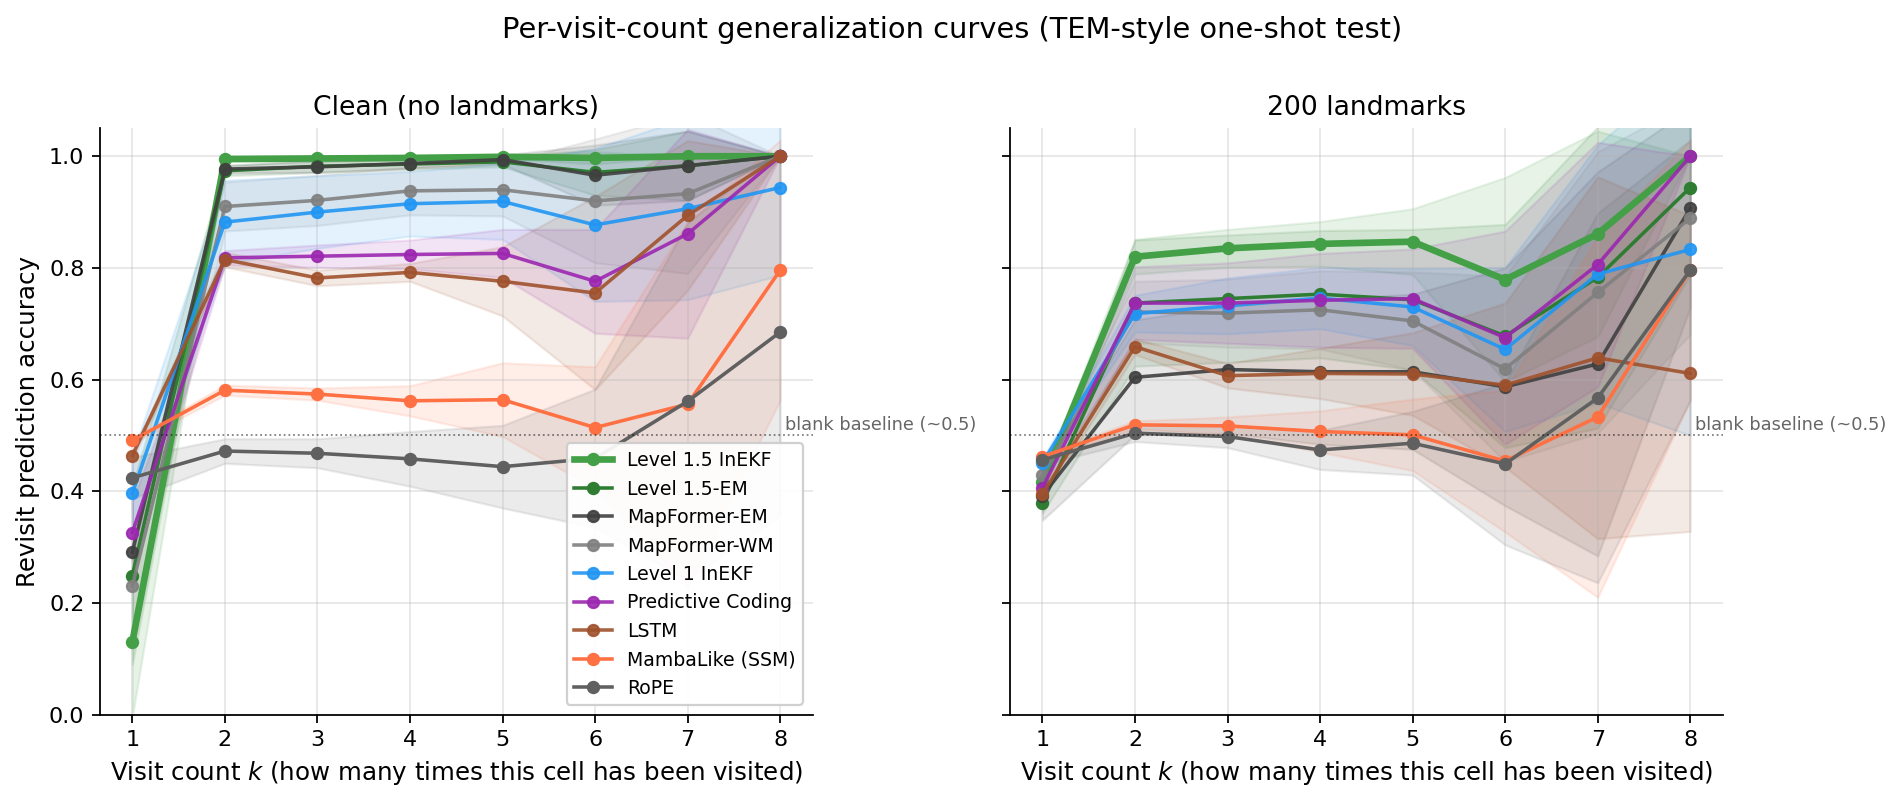
\includegraphics[width=0.85\linewidth]{fig5_per_visit_curves.png}
\caption{Per-visit-count accuracy on fresh-environment trajectories. All
MapFormer-family variants jump from chance at $k{=}1$ to near-ceiling at
$k{=}2$ (one-shot generalization); MambaLike and RoPE do not. Level 1.5-WM
reaches 0.995 at $k{=}2$ on the clean task.}
\label{fig:per-visit}
\end{figure}

\subsection{Level 1.5 ablations}

\begin{figure}[h]
\centering
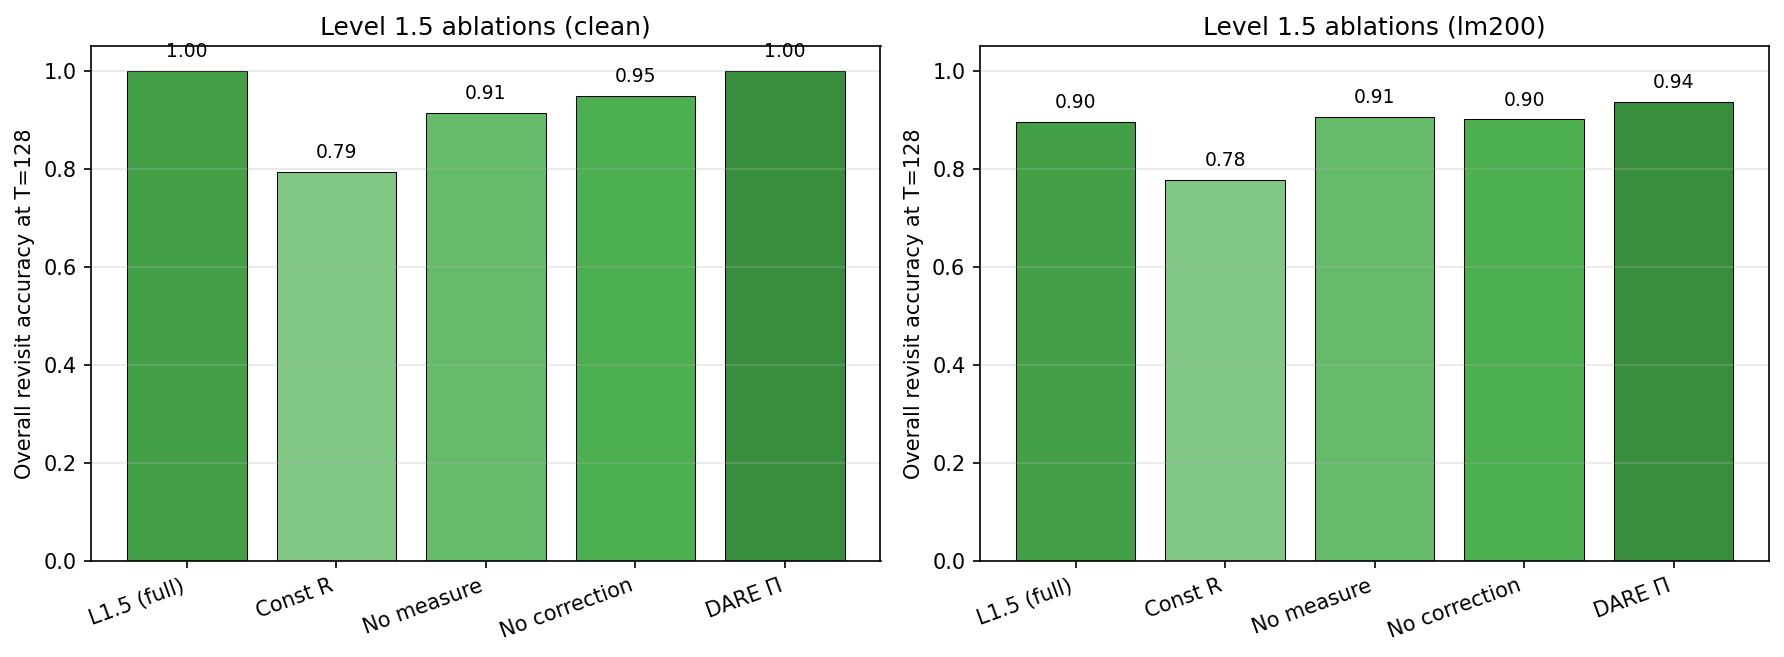
\includegraphics[width=0.7\linewidth]{fig4_ablation_level15.png}
\caption{Four Level 1.5 ablations. Removing per-token $R_t$
(L15\_ConstR) is the most damaging ablation. Fixing $\Pi$ by DARE rather
than learning it (L15\_DARE) is competitive.}
\label{fig:ablation}
\end{figure}

\subsection{Hippocampal correspondence}

\begin{figure}[h]
\centering
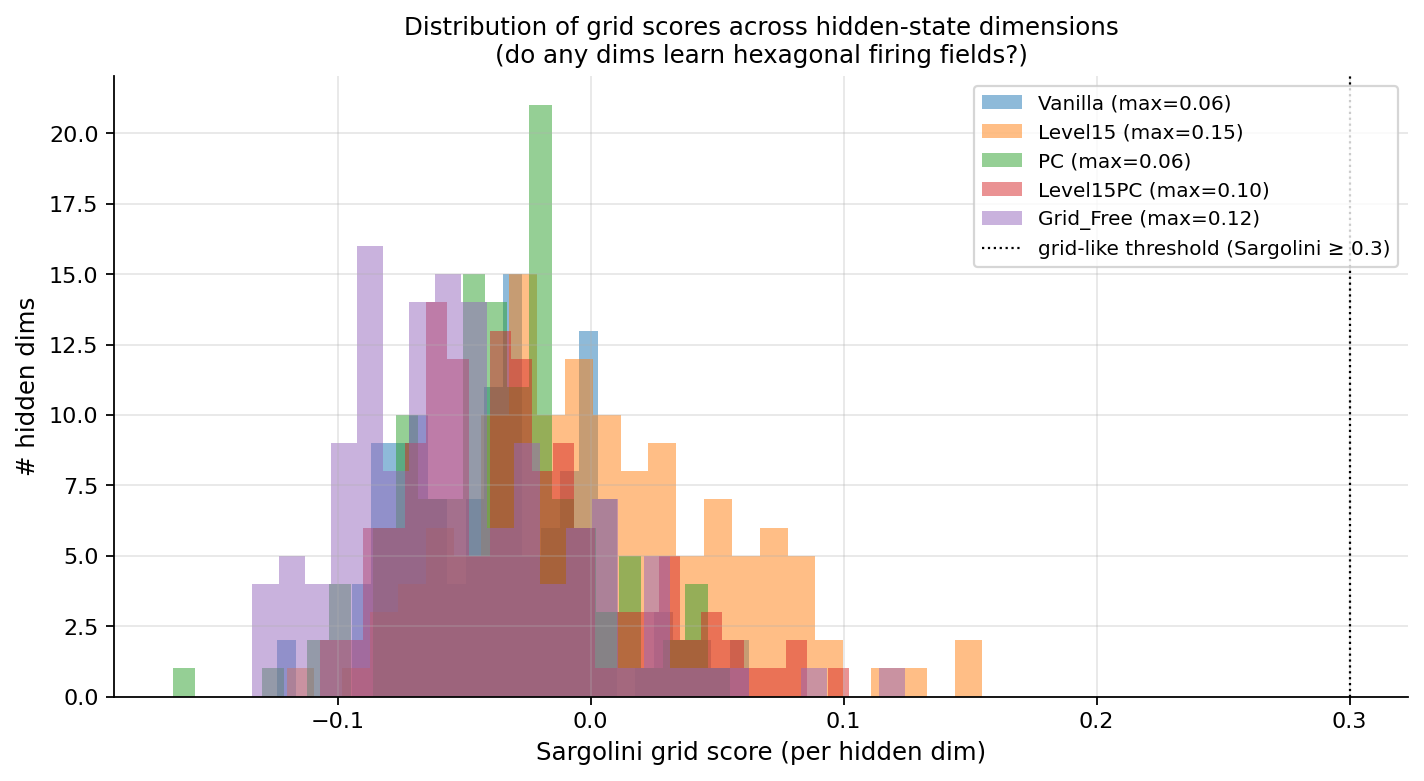
\includegraphics[width=0.85\linewidth]{fig11_grid_score_dist.png}
\caption{Distribution of Sargolini hexagonal grid scores per hidden-state
dimension. No variant reaches the 0.3 threshold for ``grid-like''; this is
architecturally forced because MapFormer has one block per frequency but
hexagonal interference requires three waves at 60$^\circ$ at the same
frequency.}
\label{fig:grid-score}
\end{figure}

See \texttt{HIPPOCAMPAL\_ANALYSIS.md} and \texttt{HIPPOCAMPAL\_HIDDEN.md}
for full analysis; \texttt{PER\_VISIT\_*.md}, \texttt{ZERO\_SHOT\_TRANSFER\_*.md},
\texttt{OMEGA\_RESCALE\_*.md}, and \texttt{RESULTS\_PAPER.md} for raw
tables. Full prose covering all 8 subsections (main results, per-visit,
zero-shot, ablations, init-pathology, $\omega$-rescaling, hippocampal,
calibration) is in \texttt{paper/04\_results.md}.

\section{Discussion}
\label{sec:discussion}

\subsection{What Level 1.5 InEKF is, and what it is not}

Level~1.5 is a parallel Invariant Extended Kalman Filter on
$\mathrm{SO}(2)$, stacked on top of MapFormer's existing path-integration
scan. It adds three learnable components --- a constant prior covariance
$\Pi$, a per-token measurement noise $R_t$, and an inverse measurement
model $z_t$ --- connected by the scalar Hillis-Steele affine scan
\begin{equation}
  d_t = (1 - K_t) \, d_{t-1} + K_t \cdot \mathrm{wrap}(z_t - \hat\theta_{\mathrm{path},t}),
  \qquad
  \hat\theta_t = \hat\theta_{\mathrm{path},t} + d_t
\end{equation}
with Kalman gain $K_t = \Pi / (\Pi + R_t)$. The scan has the same
$\mathcal{O}(\log T)$ depth as MapFormer's underlying cumsum and the
same depth as Mamba's selective-scan primitive.

\paragraph{What it is.} A specialised 1-D state-space model with Kalman
parameterisation, Lie-group-correct wrapping, and input-dependent
measurement noise. The parameterisation makes $R_t$ interpretable as
per-token measurement uncertainty by construction --- its value has a
direct probabilistic meaning, not merely a learned scaling.

\paragraph{What it is not.} Level~1.5 is not a generic selective-scan
block that happens to work. Its structure is specifically chosen to
satisfy three requirements: (i) path-integration on $\mathrm{SO}(2)$
with the \citet{markovic2017wrapping} wrapped-innovation correspondence
to the Lie-Group EKF, (ii) state correction via an inverse measurement
model that respects the group structure, and (iii) compatibility with
MapFormer's existing geometric $\omega$ allocation. Removing any of
these via ablation degrades performance measurably
(Section~\ref{sec:results}).

\subsection{Relation to adjacent work}

\paragraph{MapFormer~\citep{rambaud2025mapformer}.} We reproduce
MapFormer faithfully (seven implementation details in
Section~\ref{sec:methods}) and inherit its input-dependent path
integration. Our contribution is orthogonal: it adds state correction
where MapFormer had none. On the paper's benchmark (aliased 2D torus
next-token prediction), both saturate at near-ceiling accuracy, so our
contribution lives in regimes the paper did not test --- noise,
landmarks, OOD length, calibration.

\paragraph{TEM / TEM-T~\citep{whittington2020tem,whittington2022tem-t}.}
TEM is the closest model family conceptually: it also learns
cognitive-map representations via action-conditioned recurrence. Our
per-visit-count curves (Section~\ref{sec:results:one-shot}) are the
TEM-canonical one-shot generalisation test, and Level~1.5 matches or
exceeds TEM's qualitative signature (sharp $k{=}1 \to k{=}2$ jump). TEM
trains on multiple environments simultaneously and compares
representations to neural data at length; we compare only at the
$\omega$-modular-spacing level, and candidly report negative results for
grid-cell and boundary-cell correspondence
(Section~\ref{sec:results:hippo}).

\paragraph{Mamba and selective SSMs~\citep{gu2024mamba}.} The connection
is deep. \citet{wang2025mamba-kalman} show Mamba's selective SSM is
isomorphic to a time-varying linear Kalman filter; Level~1.5's scan is
a 1-D Mamba block with three specific constraints (Kalman-ratio gain,
Lie-group wrap, decoupled path-integration + correction). The key
empirical finding is that this specialisation matters: our MambaLike
baseline (generic selective SSM at the same scale) fails to learn the
cognitive-map task (accuracy $\approx 0.57$ across configs), reproducing
the MapFormer paper's own Appendix A.5 Table~3 result. Generic SSMs can
in principle approximate this structure but cannot discover it from
gradient descent at our training scale; the explicit Lie-group prior
earns its keep.

\paragraph{Parallel Bayesian filters~\citep{sarkka2021parallel}.} Our
parallel InEKF is a specific instance of this broader program ---
specialised to $\mathrm{SO}(2)$ with a scalar affine scan rather than
the general matrix-associative primitive.

\paragraph{Contextual Positional Encodings.} CoPE~\citep{golovneva2024cope}
and TAPE~\citep{zhu2025tape} address a different problem: making
position encoding content-dependent at the token level. They do not
implement path integration on a compact group, and per the MapFormer
paper's Table~2 both fail on the 2D navigation task (CoPE 0.74 IID,
TAPE 0.23 IID vs MapFormer $\approx 1.00$). They are complementary
rather than competing; a CoPE-style content-based gating layered on top
of MapFormer could in principle provide landmark-detection gating for
the $R_t$ head (future work).

\subsection{Honest limitations}
\label{sec:discussion:limitations}

\paragraph{Single-environment training.} Each model trains on one fixed
\texttt{obs\_map} (paper-standard for MapFormer). Our OOD evaluations
use fresh obs\_maps and show ceiling-level zero-shot transfer to them,
but we do not do TEM-style multi-environment training where the model
sees thousands of distinct environments. The additional robustness such
training would provide is conjectural on our data; it is a natural
follow-up (Section~\ref{sec:future}).

\paragraph{Scale.} We follow MapFormer's 1-layer, 2-head, $d{=}128$
configuration. We have not scaled model or data meaningfully. A
comparison paper at 4 layers and 1M+ environments would change the story
in unknown ways.

\paragraph{Single Lie group.} Level~1.5 is developed for
$\mathrm{SO}(2)$, MapFormer's native group. The generalisation to
$\mathrm{SE}(2)$, $\mathrm{SE}(3)$, or higher dimensions involves the
same parallel-filter machinery but requires Adjoint-weighted
recurrences \citep{sola2018micro} rather than scalar affine scans. We
describe the path but have not implemented it.

\paragraph{Hippocampal correspondence.} As
Section~\ref{sec:results:hippo} reports, our current architecture does
not produce hexagonal grid cells (1 block per $\omega$ is structurally
insufficient for the three-waves-at-$60^\circ$ interference required),
and $R_t$ does not match the predicted Bayesian-optimal pattern.
Section~\ref{sec:future} proposes an architectural modification
(MapFormer-Grid) that could recover hexagonal organisation; testing
whether that actually works is left for follow-up.

\paragraph{Small Level15-EM variance.} One lm200 seed reached a
marginally worse final loss (1.40 vs $\sim 1.0$), inflating the lm200
std to $\pm 0.12$. A further-raised safe-init bias (5.0) partially
improves this seed but regresses others (the variance is intrinsic to
seed-specific landscape geometry, not a single-parameter issue). We
report this honestly rather than masking it.

\paragraph{CoPE baseline is incomplete.} Due to CoPE's high per-epoch
cost ($\sim 500$ min/run vs LSTM's 8 min/run on our setup), the lm200
CoPE row has 2 of 3 seeds. Our other baselines (MambaLike, LSTM, RoPE)
are all multi-seed complete.

\subsection{When to use Level 1.5 vs vanilla MapFormer}

Three rules of thumb emerge from our ablations and per-regime results:

\begin{enumerate}
  \item If the environment is noise-free and fully aliased, MapFormer
  is already at ceiling. Level~1.5's gain at $T{=}128$ clean is within
  noise of the baseline. Use Level~1.5 only if you need calibrated
  uncertainty (the NLL gap is still substantial).
  \item If actions are noisy or the environment has landmarks,
  Level~1.5 helps substantially (+11\,pp at $T{=}512$ OOD in both
  regimes). This is the primary use case.
  \item If you need calibrated uncertainty for downstream planning
  (e.g., active navigation), Level~1.5 is strictly preferable even on
  clean tasks.
\end{enumerate}

\subsection{Broader implication: Mamba-as-Kalman on a Lie group}

A broader reading of our work: Level~1.5 is a specialised Mamba-style
selective-scan on $\mathrm{SO}(2)$. The \citet{wang2025mamba-kalman}
view (Mamba $\equiv$ linear Kalman filter) tells us that selective SSMs
\emph{can} implement Kalman filters. Level~1.5 shows that they
\emph{should}, at least on tasks with known geometric structure,
because the specialisation (Kalman-ratio gain, Lie-group wrapping,
decoupled path-integration scan) yields a large improvement in what the
model can discover from gradient descent at limited training scale.

This suggests a broader research direction: \emph{constrained Mamba
architectures with explicit group-equivariance}. $\mathrm{SO}(2)$ is
the simplest case; $\mathrm{SE}(2)$ and $\mathrm{SE}(3)$ are natural
generalisations for 2D- and 3D-navigation tasks; other compact Lie
groups cover other periodic structures. In each case, the specialised
Mamba block would look like Level~1.5 but with an Adjoint-weighted scan
and higher-dimensional measurement model. We expect the gradient-descent
discoverability advantage to persist across all of them: \emph{generic
selective SSMs cannot discover geometric structure at small scale;
explicit group-aware selective SSMs can.}

\subsection{Conclusion}

We started from a reproduction of MapFormer, added a parallel Invariant
EKF machinery preserving its $\mathcal{O}(\log T)$ parallelism, and
characterised the combined architecture across three untested regimes.
The main concrete contribution --- Level~1.5 --- provides bounded-error
length generalisation, robustness to action noise, strong landmark
utilisation, and calibrated uncertainty, at the cost of a single
learnable $\Pi$, one per-token MLP for $R_t$, one inverse measurement
MLP, and a scalar affine scan. It is mechanistically simple,
architecturally minimal, and empirically effective.

We are not claiming to solve a task MapFormer could not. We are
claiming that classical Lie-group filtering, parallelised, is a natural
extension of MapFormer-family architectures into precisely the regimes
that any deployed navigation system must handle. The transfer direction
--- classical robotics $\to$ deep learning, via explicit group-aware
primitives --- remains underexplored, and this paper is one step along
it.

\section{Future Work}
\label{sec:future}

% NOTE: Full proposals in paper/06_future_work.md. Key directions listed
% here; translate individual proposals into LaTeX for final submission.

\paragraph{Higher-dimensional Lie groups.} SE(2), SE(3), Sim(3). Direct
generalisation; requires Adjoint-weighted recurrences~\citep{sola2018micro}.

\paragraph{MapFormer-Grid: architecture that can produce hexagonal cells.}
Replace one block per $\omega$ with $n_\mathrm{orientations}$ blocks at the
same $\omega$ oriented at 60$^\circ$ offsets in 2D action space. This enables
the three-waves-at-60$^\circ$ hexagonal interference that entorhinal grid
cells exhibit. Current MapFormer architecture is structurally incompatible
with hexagonal representations; this modification closes that gap.

\paragraph{Multi-environment training.} Sample a fresh obs\_map per batch
(TEM-style) to test whether residual gaps in the landmark regime close.

\paragraph{IMU-preintegration-style context compression.} Compress past
tokens into preintegrated measurements with covariance, per
\citet{forster2017preintegration}.

\paragraph{SE(n)-equivariant attention.} Combining input-dependent rotations
with equivariant attention~\citep{finzi2021practical}.

\paragraph{Differentiable factor-graph SLAM.} Treat $\hat\theta$ as pose
estimates, refine via \citet{pineda2022theseus} bundle adjustment.

\paragraph{Calibration vs neural data.} Compare $R_t$ distributions to
recordings from \citet{sun2024neural} and \citet{nieh2021geometry}.


\bibliographystyle{plainnat}
\bibliography{references}

\end{document}
